\documentclass{beamer}
\usetheme{Madrid}

%\usepackage[colorlinks,linkcolor=blue]{hyperref}
\usepackage{german}
\usepackage{listings}
\documentclass[11pt]{ctexart}  
\usepackage[top=2cm, bottom=2cm, left=2cm, right=2cm]{geometry}  
\usepackage{algorithm,algorithmic}

\title{Karatsuba Algorithmus}
\author{by Qianli Wang}
\centering
\date{16.06.2020}
\begin{document}
\maketitle
\begin{frame}{Gliederung}
\begin{itemize}
\item Einführung
\item Addition zweier Zahlen mit Länge n
\item Multiplikation einer Zahl mit einer Ziffer
\item Grundschulmethode zur Multiplikation
\item Karatsuba Algorithmus
\item Zusammenfassung
\item Literatur
\end{itemize}
\end{frame}

\floatname{algorithm}{算法}  

\begin{frame}{Einführung}
\framesubtitle{Warum Multiplikation? Warum Karatsuba Algorithmus?}
\begin{itemize}
    \onslide<1,2,3>\item In der Grundschule gelernt. 
    \onslide<2,3>\item \textbf{Anwendungen:} Verschlüssung von Nachrichten, Kryptographie, polynomielle Multiplikation oder Lösung von geometrischen Problemen usw. 
    \onslide<3>\item Ineffizient bei der Multiplikation zweier großen Zahlen.
\end{itemize}
\end{frame}
\begin{frame}{Vordefinition}
    \onslide<1,2>\begin{block}{\textbf{Definition 1:}}
    Eine \textbf{Grundoperation} ist eine Operation, die der Prozessor direkt unterstützt. z.B. Addition, Multiplikation
    \end{block}
    
    \onslide<2>\begin{block}{\textbf{Beobachtung 2: }}
    Die zifferweise Addition und Multiplikation kostet nur konstante Zeit, also $\mathcal{O}(1)$.
    \end{block}
\end{frame}

\begin{frame}{Vorbemerkung}
    %%wenn ich später so eine Zahl mit Länge n sage, ist die Länge von entsprechendem Array gemeint.  
    \begin{block}{Vorbemerkung:}
    Wir können eine Zahl als ein Array von Ziffern betrachten:\\
    12345 $\rightarrow$ ['1', '2', '3', '4', '5']\\
    Anzahl von Ziffern $\Leftrightarrow$ Länge vom Array
    \end{block}
\end{frame}

\begin{frame}{Addition zweier Zahlen mit Länge n}
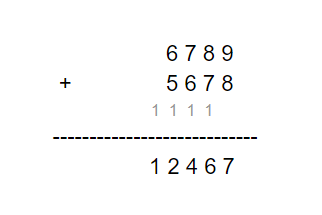
\includegraphics[scale = 0.7]{addition.png}\\

\begin{block}{Schritte:}
    \begin{itemize}
      \onslide<1,2,3,4>\item[1)] Schreiben die beiden Zahlen untereinander
      \onslide<2,3,4>\item[2)] Gehen von rechts nach links alle Spalten durch und rechnen.
      \onslide<3,4>\item[3)] Tragen Überträge eine Stelle davor
      \onslide<4>\item[4)] Schreiben den letzten Übertrag als linkeste Ziffer des Ergebnis hin.
  \end{itemize}
\end{block}
 
\end{frame}

\begin{frame}
\frametitle{Analyse von der Addition}
\onslide<1,2>\begin{itemize}
    \item \textbf{Angenommen: } Wir haben zwei Zahlen mit Länge n. 
\end{itemize}
\onslide<1,2>\begin{block}{Satz 3: }
Die Addition zweier Zahlen benötigt $n$ Grundoperationen. Die Laufzeit liegt in $\mathcal{O}(n)$
\end{block}
 
\onslide<2>\begin{block}{Beweis: }
Die Länge n entspricht dann n ziffernweise Additionen. Man bekommt die linkeste Ziffer ohne weitere Berechnung. \\
$ \rightarrow $ Laufzeit:  $\mathcal{O}(n)$.
\end{block}
\end{frame}

\begin{frame}{Multiplikation einer Zahl mit einer Ziffer}
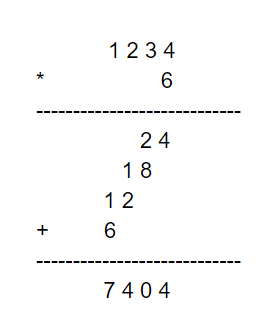
\includegraphics[scale = 0.4]{multiplication with digit.png}\\
\begin{block}{Schritte}
    \begin{itemize}
        \onslide<1,2,3>\item[1)] Berechne alle Teilprodukte von zifferweise jeweiligen Multiplikationen.
        \onslide<2,3>\item[2)] Schreiben Teilprodukte von rechts nach links schräg auf.
        \onslide<3>\item[3)] Addieren alle Ziffer in der selben Spalte. 
    \end{itemize}
\end{block}
\end{frame}

\begin{frame}{Analyse}
\begin{itemize}
    \item  \textbf{Angenommen:} a ist eine Zahl mit Länge n, b ist eine Ziffer. 
\end{itemize}
    \onslide<1,2>\begin{block}{Satz 4: }
    Laufzeit der Multiplikation einer Zahl mit einer Ziffer ist $\mathcal{O}(n)$. Die Multiplikation braucht 2n Grundoperationen.
    \end{block}
    
    \onslide<2>\begin{block}{Beweis: }
    Jeder Ziffer von a soll jeweils einmal mit b multiplizieren\\ $\rightarrow$ n Multiplikationen.\\ Anschließend sollen alle Teilprodukte addiert werden $\rightarrow$ n Additionen. \\
    $\rightarrow$ Insgesamt 2n Grundoperationen.\\
    $\rightarrow Laufzeit: \mathcal{O}(n)$
    \end{block}
\end{frame}

\begin{frame}{Grundschulmethode zur Multiplikation}
\begin{itemize}
    \item \textbf{Als Beispiel:} Wir haben zwei Zahlen 1234 und 5678, die beiden aus 4 Ziffern bestehen. 
\end{itemize}
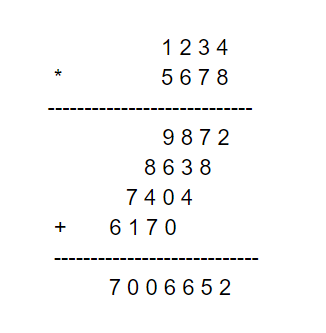
\includegraphics[scale = 0.6]{example_of_school_multiplcation.png}
\centering\\
\begin{block}{Schritte}
\begin{itemize}
    \onslide<1,2>\item[1)] Es werden die Teilprodukte nebeneinander geschrieben. 
    \onslide<2>\item[2)] Beginnt mit der niedrigsten Stelle und man kann es danach leicht  addieren. 
\end{itemize}
\end{block}
\end{frame}

\begin{frame}{Analyse von Grundoperationen}
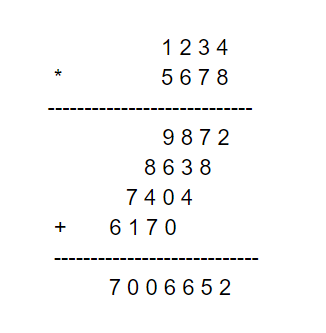
\includegraphics[scale = 0.6]{example_of_school_multiplcation.png}
\begin{block}{Analyse von der Multiplikation:}
\begin{itemize}
    \item[1)] ``Zahl mal Ziffer`` Multiplikation
    \item[2)] n solche Multiplikationen notwendig 
\end{itemize}
$\rightarrow$ Anzahl der Grundoperationen = $2n \cdot n = 2n^2$
\end{block}
    
\end{frame}

\begin{frame}{Analyse von Grundoperationen}
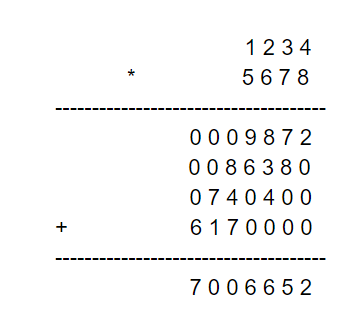
\includegraphics[scale = 0.5]{advance.png}
\begin{block}{Analyse von der Addition:}
\begin{itemize}
    \item[1)] Teilprodukt kann max. $(n + 1)$ Ziffern haben. 
    \item[2)] Höchstens $(n + 1 + n - 1) = 2n$ spaltenweise Additionen 
\end{itemize}
$\rightarrow$ Anzahl der Grundoperationen zur Addition = $2n \cdot (n - 1) = 2n^2 - 2n$\\
$\Rightarrow$ Sämtliche Anzahl der Grundoperationen = $2n^2 - 2n + 2n^2 = 4n^2 - 2n$
$\Rightarrow Laufzeit: \mathcal{O}(n^2)$
\end{block}
    
\end{frame}

\begin{frame}{Teile und Herrsche}
\begin{figure}[!ht]  
    \centering  
    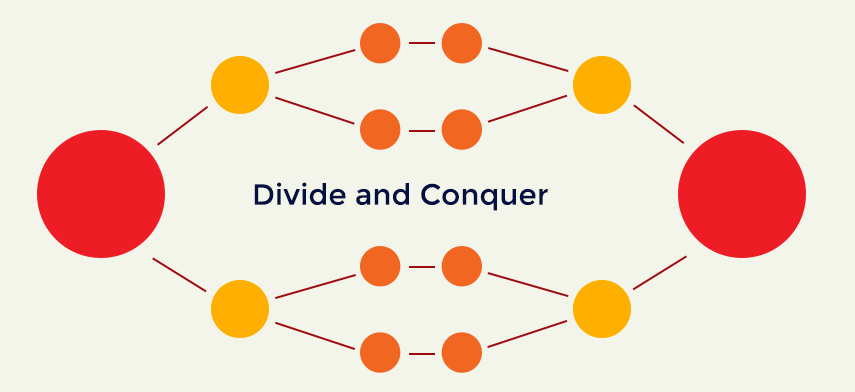
\includegraphics[scale = 0.2]{divide and conquer.png}
    \caption{\footnotesize Quelle: \  \textcolor{blue}{ \href{https://medium.com/@gaurav_52429/divide-and-conquer-paradigm-in-algorithms-ef43fb2222f5}{https://medium.com/@gaurav\_52429/divide-and-conquer-paradigm-in-algorithms-ef43fb2222f5}}}  
\end{figure} 
\begin{block}{Definition: }
\textbf{Teile und Herrsche} zerlegt ein Problem rekursiv in zwei oder mehrere Unterprobleme desselber oder verwandter Art, bis diese einfach genug werden, um dirkt gelöst werden zu können. 
\end{block}
\end{frame}



\begin{frame}{Splitmultiply}
\begin{itemize}
    \item \textbf{Angenommen,}dass wir zwei Zahlen p und q haben mit Länge n. Wir definieren $m = \lfloor \frac{n}{2} \rfloor$. Dann können wir p und q so darstellen:
\end{itemize}
    \begin{align*}
        p = 10^{m} \cdot a + b\\
        q = 10^{m} \cdot c + d\\
        (wobei \;a, \;b, \;c, \;d \in \mathbb{Z})
    \end{align*}    
    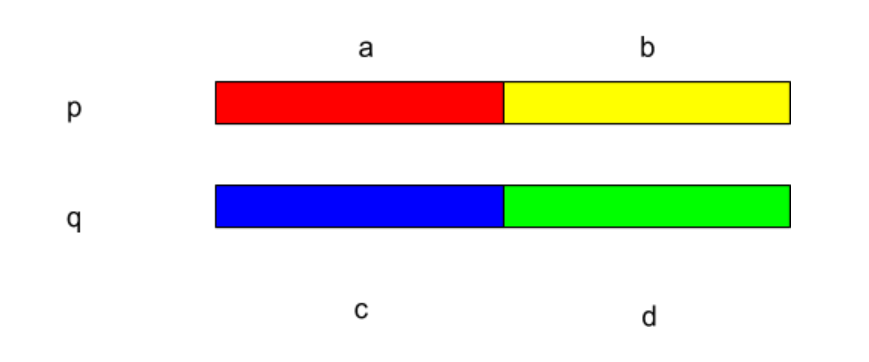
\includegraphics[scale = 0.5]{color.png}
\end{frame}

\begin{frame}{Darstellung von p und q}
    \begin{itemize}
        \item \textbf{Distributivitätsgesetz} verwenden:
    \end{itemize}
    \begin{align}
    p \cdot q &= (10^{m} \cdot a + b) \cdot (10^{m} \cdot c + d)\\
    &= a \cdot c \cdot 10^{2m} + (a \cdot d + b \cdot c) \cdot 10^{m} + b \cdot d\\
    &= a \cdot c \cdot 10^{n} + (a \cdot d + b \cdot c) \cdot 10^{\frac{n}{2}} + b \cdot d
    \end{align}
\end{frame}

\begin{frame}{Pseudocode}
\begin{algorithm}[H]                           % HERE!!!!!!!!!
\caption{SPLITMULTIPLY(x, y, n):}          % give the algorithm a caption
\label{alg1}      % and a label for \ref{} commands later in the document
\begin{algorithmic}  % enter the algorithmic environment
\REQUIRE $n \geq 1 $
\ENSURE $Get \ the \ correct \ product \ of \ x \ and \ y$

\IF{$n = 1$}
\STATE $return \quad x \cdot y$
\ELSE
\STATE $m \leftarrow \lfloor \frac{n}{2} \rfloor$
\STATE $a \leftarrow \lfloor \frac{x}{10^m} \rfloor; \quad  b \leftarrow x \ mod \ 10^m; \quad c \leftarrow \lfloor \frac{y}{10^m} \rfloor; \quad d \leftarrow y \ mod \ 10^m$
\STATE $e \leftarrow SPLITMULTIPLY(a, c, m)$
\STATE $f \leftarrow SPLITMULTIPLY(b, d, m)$
\STATE $g \leftarrow SPLITMULTIPLY(b, c, m)$
\STATE $h \leftarrow SPLITMULTIPLY(a, d, m)$
\STATE $return \quad 10^{2m} \cdot e + 10^{m}(g+h) + f$
\ENDIF
\end{algorithmic}
\end{algorithm}
\end{frame}

\begin{frame}{Analyse}
\begin{itemize}
    \item $p \cdot q = a \cdot c \cdot 10^{n} + (a \cdot d + b \cdot c) \cdot 10^{\frac{n}{2}} + b \cdot d \quad (3)$
\end{itemize}
\onslide<1,2>\begin{block}{Beobachtung 5: }
4 unterschiedlichen Multiplikationen mit Länge $\lfloor \frac{n}{2} \rfloor$ erforderlich.\\ Darüber hinaus sind 3 Additionen mit Länge $\lfloor \frac{n}{2} \rfloor$ benötigt.
\end{block}

\onslide<2>\begin{block}{Satz 6: }
Laufzeit des einfachen divide and conquer Ansatzes ist $\mathcal{O}$($n^{2}$).
\end{block}
\end{frame}

\begin{frame}{Analyse}
\begin{block}{Beweis vom Satz 6: }
$\rightarrow$ 4 Multiplikationen braucht. Dann können wir die Rekursionsformel so formulieren: \\
\quad		T(n) = 4 $\cdot$ T$(\lfloor \frac{n}{2}\rfloor)$ + $\mathcal{O}(n)$\\
\quad		T($\frac{n}{2}$) = 4 $\cdot$ T($\lfloor \frac{n}{4}\rfloor$) + $\mathcal{O}$($\frac{n}{2}$)\\
\quad		...\\
\quad		T(2) = 4 $\cdot$ T(1) + $\mathcal{O}(1)$ \quad (wobei T(1) = $\mathcal{O}$(1))\\
\end{block}
\end{frame}

\begin{frame}{Beweis der Rekursionsformel}
\begin{figure}[!ht]  
    \centering  
    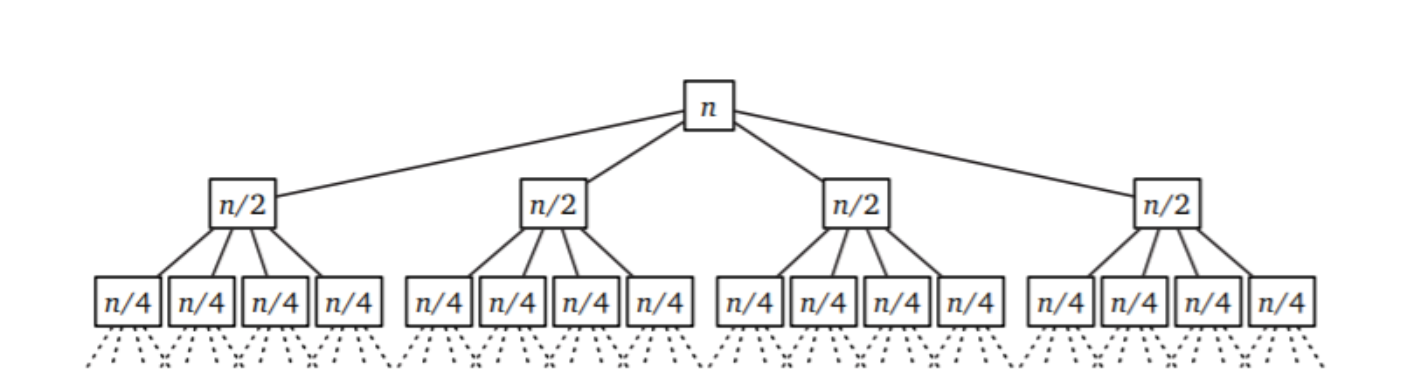
\includegraphics[scale = 0.3]{baum.png}
    \caption{\footnotesize Quelle: \  \textcolor{blue}{ \href{http://jeffe.cs.illinois.edu/teaching/algorithms/book/Algorithms-JeffE.pdf}{http://jeffe.cs.illinois.edu/teaching/algorithms/book/Algorithms-JeffE.pdf}}}  
\end{figure}  


\begin{block}{Beweis: }
Tiefe: $log_{2}{n}$.  
Auf der \textbf{ersten} Ebene: $4^{1}$ Rekursionen. Auf der \textbf{zweiten} Ebene: $4^{2}$ Rekursionen, usw. Das heißt, auf der \textbf{letzten} Ebene gibt es dann $4^{\log_2{n}}$ Rekursionen. Und die Laufzeit jeder Rekursion auf der letzten Ebene ist $T(1) \ bzw. \ \mathcal{O}(1)$.\\
$\rightarrow \quad$ Laufzeit: $4^{\log_{2}{n}} \cdot \mathcal{O}(1) = $ $ \mathcal{O}( 4^{\log_{2}{n}}) = \mathcal{O}(n^{\log_{2}{4} }) = \mathcal{O} (n^{2})$\\
\end{block}
\end{frame}

\begin{frame}{Einführung vom Karatusba Algorithmus}
\begin{figure}[!ht]  
    \centering  
    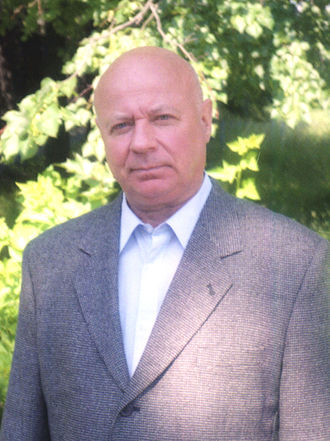
\includegraphics[scale = 15]{330px-Anatolii_Karatsuba.jpg}
    \caption{\footnotesize Quelle: \  \textcolor{blue}{ \href{https://en.wikipedia.org/wiki/Anatoly_Karatsuba}{https://en.wikipedia.org/wiki/Anatoly_Karatsuba}}}  
\end{figure}  

\begin{itemize}
    \onslide<1,2,3,4>\item Von Anatoli Alexejewitsch Karazuba in 1962 veröffentlicht
    \onslide<2,3,4>\item Schneller als die quadratische Grundschulmethode
    \onslide<3,4>\item Laufzeit: $\mathcal{O}(n^{\log_2{3}}) \approx \mathcal{O}(n^{1.585})$
    \onslide<4>\item Eine Multiplikation eingespart
\end{itemize}
\end{frame}

\begin{frame}{Vorbereitung}
    \onslide<1,2,3>\begin{block}{Kernidee:}
    4 Unterprobleme auf 3 Unterproblemen reduzieren.
    \end{block}
    
    \onslide<2,3>\begin{block}{Fallunterscheidung von den Eingaben:}
    \textbf{Fall 1: }Multiplikation zweier einstelligen Zahlen (n = 1).\\
    \textbf{Fall 2: }Multiplikation zweier Zahlen mit Länge n, wobei n größer 1 ist.
    \end{block}
    
    \onslide<3>\begin{block}{Beobachtung 7}
    Im ersten Fall kann man sofort Ergebnis bekommen, weil dafür genau nur eine Grundoperation benötigt ist, die vom Prozessor direkt unterstützt ist.
    \end{block}
\end{frame}

\begin{frame}{Karatsuba Algorithmus}
\onslide<1,2>\begin{block}{Umformen:}
Wir haben zwei Zahlen p und q mit Länge n und definieren $m = \lfloor \frac{n}{2} \rfloor$.\\
\begin{align*}
        p = 10^{m} \cdot a + b\\
        q = 10^{m} \cdot c + d\\
        (wobei \;a, \;b, \;c, \;d \in \mathbb{Z})
    \end{align*}    
Dann können wir $p \cdot q$ so formulieren:  
\onslide<2>\begin{align*}
p \cdot q &= (10^{m} \cdot a + b) \cdot (10^{m} \cdot c + d)\\
                 &= a \cdot c \cdot 10^{2m} + (a \cdot d + b \cdot c) \cdot 10^{m} + b \cdot d \quad (Formel 3)\\
				 &= a\cdot c\cdot 10^{2m} + (a \cdot c + b \cdot d - (b - a) \cdot (d - c)) \cdot 10^{m} + b \cdot d\\
				 &= a\cdot c\cdot 10^{n} + (a \cdot c + b \cdot d - (b - a) \cdot (d - c)) \cdot 10^{\frac{n}{2}} + b \cdot d
\end{align*}
\end{block}    
\end{frame}

\begin{frame}{Karatsuba Algorithmus}
    \begin{block}{Beweis der Korrektheit vom Umformen:}
$        (a \cdot c + b \cdot d - (b - a) \cdot (d - c))$\\
$= a \cdot c + b \cdot d - (b \cdot d - b \cdot c - a \cdot d + a \cdot c)$\\
$= a \cdot c + b \cdot d - b \cdot d + b \cdot c + a \cdot d - a \cdot c$\\
$= b \cdot c + a \cdot d $ 
    \end{block}
\end{frame}

\begin{frame}{Karatsuba Algorithmus}
\begin{block}{Genauere Beschreibung: }
Seiene: 
\begin{align*}
u &= a \cdot c\\
v &= (b - a) \cdot (d - c)\\
w &= b \cdot d
\end{align*}
Also wir können $p \cdot q$ als folgendes umschreiben: 
\begin{align*}
p \cdot q = u \cdot 10^{n} + (u + w - v) \cdot 10^{\frac{n}{2}} + w
\end{align*}
$\rightarrow$ Eine Multiplikation eingespart.
\end{block}
\end{frame}

\begin{frame}{Karatsuba Algorithmus}
    \begin{block}{Beispiel: }
    Wir wollen das Produkt von 12345 und 6789 berechnen. Seien a = 12, b = 345 und c = 6, d = 789, nämlich:
\begin{align*}
12345 &= 12 \cdot 1000 + 345\\
6789 &= 6 \cdot 100 + 789
\end{align*}
Zwischenergebnisse:
\begin{align*}
&u = a \cdot c = 12 \cdot 6 = 72\\
&v = (b - a) \cdot (d - c) = (345 - 12) \cdot (789 - 6) = 260739\\
&w = b \cdot d = 345 \cdot 789 = 272205
\end{align*}
$\Rightarrow 12345 \cdot 6789 = u \cdot 10^{6} + (u + w - v) \cdot 10^{3} + v = 83810205$
    \end{block}
\end{frame}

\begin{frame}{Pseudocode}
\begin{algorithm}[H]                           % HERE!!!!!!!!!
\caption{karatsuba(num1, num2):}          % give the algorithm a caption
\label{alg1}      % and a label for \ref{} commands later in the document
\begin{algorithmic}  % enter the algorithmic environment
\REQUIRE $The \ length \ of \ each \ number \ is \geq \ 1.$
\ENSURE $Get \ the \ correct \ product \ of \ num1 \ and \ num2$

\IF{$(num1 < 10) \ or \ (num2 < 10)$}
\STATE $return \ num1 \cdot num2$
\ELSE
\STATE $m \leftarrow max(size\_base10(num1), size\_base10(num2))$
\STATE $m_2 \leftarrow floor(m / 2) $
\STATE $high1, low1 \leftarrow split\_at(num1, m_2)$
\STATE $high2, low2 \leftarrow split\_at(num2, m_2)$
\STATE $u \leftarrow karatsuba(high1, high2)$
\STATE $v \leftarrow karatsuba((high1-low1), (high2-low2))$
\STATE $w \leftarrow karatsuba(low1, low2)$
\STATE $return \quad (u \cdot 10^{m_2 \cdot 2}) + ((u + w - v) \cdot 10 ^{m_2}) + w$
\ENDIF
\end{algorithmic}
\end{algorithm}
\end{frame}

\begin{frame}{Laufzeitsanalyse}
    \onslide<1,2,3>\begin{block}{Beobachtung 9}
    Außer den Multiplikationen werden noch $\mathcal{O}(n)$ Additionen benötigt.
    \end{block}
    
    \onslide<2,3>\begin{block}{Satz 10}
    Die Laufzeit von Karatsuba Algorithmus ist $\mathcal{O}$($n^{\log_{2}{3}}$).
    \end{block}
    
    \onslide<3>\begin{block}{Beweis}
    \textbf{Initialisierung: } T(1) = $\mathcal{O}$(1)\\
    \textbf{Rekursionsformel:}  $T(n) = 3 \cdot T(\frac{n}{2}) + \mathcal{O}(n)$\\
    \textbf{Angenommen: } n = $2^{k}$ \Leftrightarrow \ $\log_{2}{n} = k$\\
    $\Rightarrow$ $f(k)$ = T($2^{k}$)\\
    \end{block}
\end{frame}

\begin{frame}{Laufzeitsanalyse}
    \begin{block}{Beweis:}
    \begin{align*}
        &\Rightarrow \ f(k) = 3 \cdot \ f(k - 1) + 2^{k}\\
        &\Leftrightarrow \ \frac{f(k)}{3^k} = \frac{f(k - 1)}{3^{k-1}} + (\frac{2}{3})^{k}\\
        &\Rightarrow \ f(k) \leqslant \ 3^{k+1} \quad (*) \\ 
    \end{align*}
\begin{equation*}
\textbf{Dann können wir die in die Definition von f einsetzen:} \\
&T(n) = T(2^{k}) = f(k) = f(\log_{2}{n}) \leqslant \ 3^{\log{2}{n}+1}\\
&\Rightarrow \ T(n) = \mathcal{O}(3^{\log_{2}{n}}) = \mathcal{O}(2^{\log_{2}{3} \cdot \log_{2}{n}}) = \mathcal{O}(n^{\log_{2}{3}})
\end{equation*}
    \end{block}
\end{frame}

\begin{frame}{Beweis}
    \begin{block}{(*)}
    \begin{align*}
        \frac{f(k)}{3^{k}} &= \frac{f(k - 1)}{3^{k-1}} + (\frac{2}{3})^{k}\\
        \frac{f(k-1)}{3^{k-1}} &= \frac{f(k - 2)}{3^{k-2}} + (\frac{2}{3})^{k-1}\\
        ...\\
        \frac{f(1)}{3^{1}} &= \frac{f(0)}{3^{0}} + (\frac{2}{3})^{1}\\
    & \Rightarrow \frac{f(k)}{3^{k}} - \frac{f(0)}{3^{0}} = \sum_{i = 1}^{k}(\frac{2}{3})^{i} = \frac{\frac{2}{3} \cdot (1-\frac{2}{3})^k}{1-\frac{2}{3}} = \frac{2}{3^k} \\
    & \Leftrightarrow \ f(k) \ = \ 3^{k} \cdot (1 + 2 \cdot \frac{1}{3^{k}}) = 3^{k} + 2\\    
    & \Rightarrow \ f(k) \leqslant \ 3^{k+1}
    \end{align*}
    \end{block}
\end{frame}

\begin{frame}{Laufzeitsvergleich}
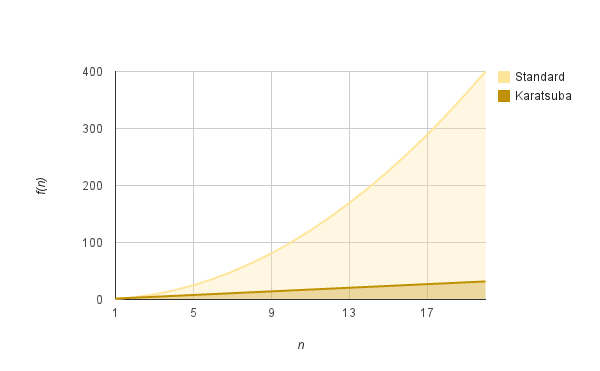
\includegraphics[scale = 0.4]{Karatsuba-Complexity.png}
    \setlength{\tabcolsep}{7mm}
\begin{tabular}{|c|c|c|}
	\hline
	Länge & Karatsuba & Grundschulmethode\\
	\hline
	1,024=$2^{10}$ &  59,049 &  1,048,675\\
	\hline
	1,048,576 = 2^{20} & 3,486,784,401 & 1,099,511,627,776\\
	\hline
	$n = 2^k$ & $3^k$ & $4^k$\\
	\hline
\end{tabular}\\
\end{frame}

\begin{frame}{Schlussfolgerung}
\begin{itemize}
    \item Wenn die Zahlen ziemlich lang sind, ist Karatsuba Algorithmus viel besser.
    \item Ab welcher Länge?
\end{itemize}
\end{frame}

\begin{frame}{Andere Methoden}
\begin{itemize}
    \item[1)] \textbf{Schönhage-Strassen-Algorithmus} in $\mathcal{O}(n \cdot \log{n} \cdot \log{\log{n}})$ (FTT)\\
    \footnotesize{$(Quelle: https://de.wikipedia.org/wiki/Sch\%C3\%B6nhage-$\\$Strassen-Algorithmus)$}
    \item[2)]
	\textbf{Toom-Cook-Algorithmus} in $\mathcal{O}(n \cdot \log{n} \cdot 2^{\sqrt{log{(n)}}})$\\
	\footnotesize{(Quelle: $https://de.wikipedia.org/wiki/Toom-Cook-Algorithmus)$}
\end{itemize}
\end{frame}

\begin{frame}{Zusammenfassung}
    \begin{itemize}
        \item Multiplikation auf kleinere Unterprobleme zurückführen\\ $\rightarrow$ Divide and Conquer
        \item 3 anstatt 4 Multiplikationen
        \item Laufzeit: $\mathcal{O}$($n^{\log_{2}{3}}$)
    \end{itemize}
\end{frame}

\begin{frame}{Literatur}
\begin{itemize}
    \item $https://en.wikipedia.org/wiki/Karatsuba\_algorithm$
    \item $https://iq.opengenus.org/content/images/2018/05/Karatsuba-Complexity.png$
    \item $https://de.wikipedia.org/wiki/Sch\%C3\%B6nhage-$\\$Strassen-Algorithmus$
\item $https://de.wikipedia.org/wiki/Toom-Cook-Algorithmus$
\end{itemize}
    
\end{frame}

\begin{frame}
\huge{\centerline{Vielen Dank für Ihre Aufmerksamkeit!}}
\end{frame}

\end{document}
